\chapter{Aromaticity and Electrophilic Aromatic Substitution}\label{ch:b2:aromatic-substitution}

Bromine water loses its colour within seconds when shaken with an alkene,
and not at all with benzene. Yet benzene does react with bromine once a
little iron(III) bromide is added --- and the product, bromobenzene, still
has its six-membered \omterm{def:b2:huckel:aromatic}{aromatic} ring: one hydrogen has been replaced, nothing
has been added. \omterm{def:b2:huckel:aromatic}{Aromatic} rings substitute rather than add, because addition
would throw away the stabilisation computed in \cref{ch:b2:huckel}. The same
mechanism nitrates, sulfonates, alkylates and acylates benzene rings, and
the groups already on a ring decide, with surprising regularity, where the
next one goes.

\begin{recall}
\Cref{ch:b2:huckel}: aromaticity and the \omterm{def:b2:huckel:delocalisation}{delocalisation energy} of benzene. The Year 1
volume: electrophilic additions to alkenes, inductive and mesomeric effects, donor and
acceptor groups, carbocations and their rearrangements, the Hammond postulate, Lewis acids,
energy profiles.
\end{recall}

\begin{omfigure}
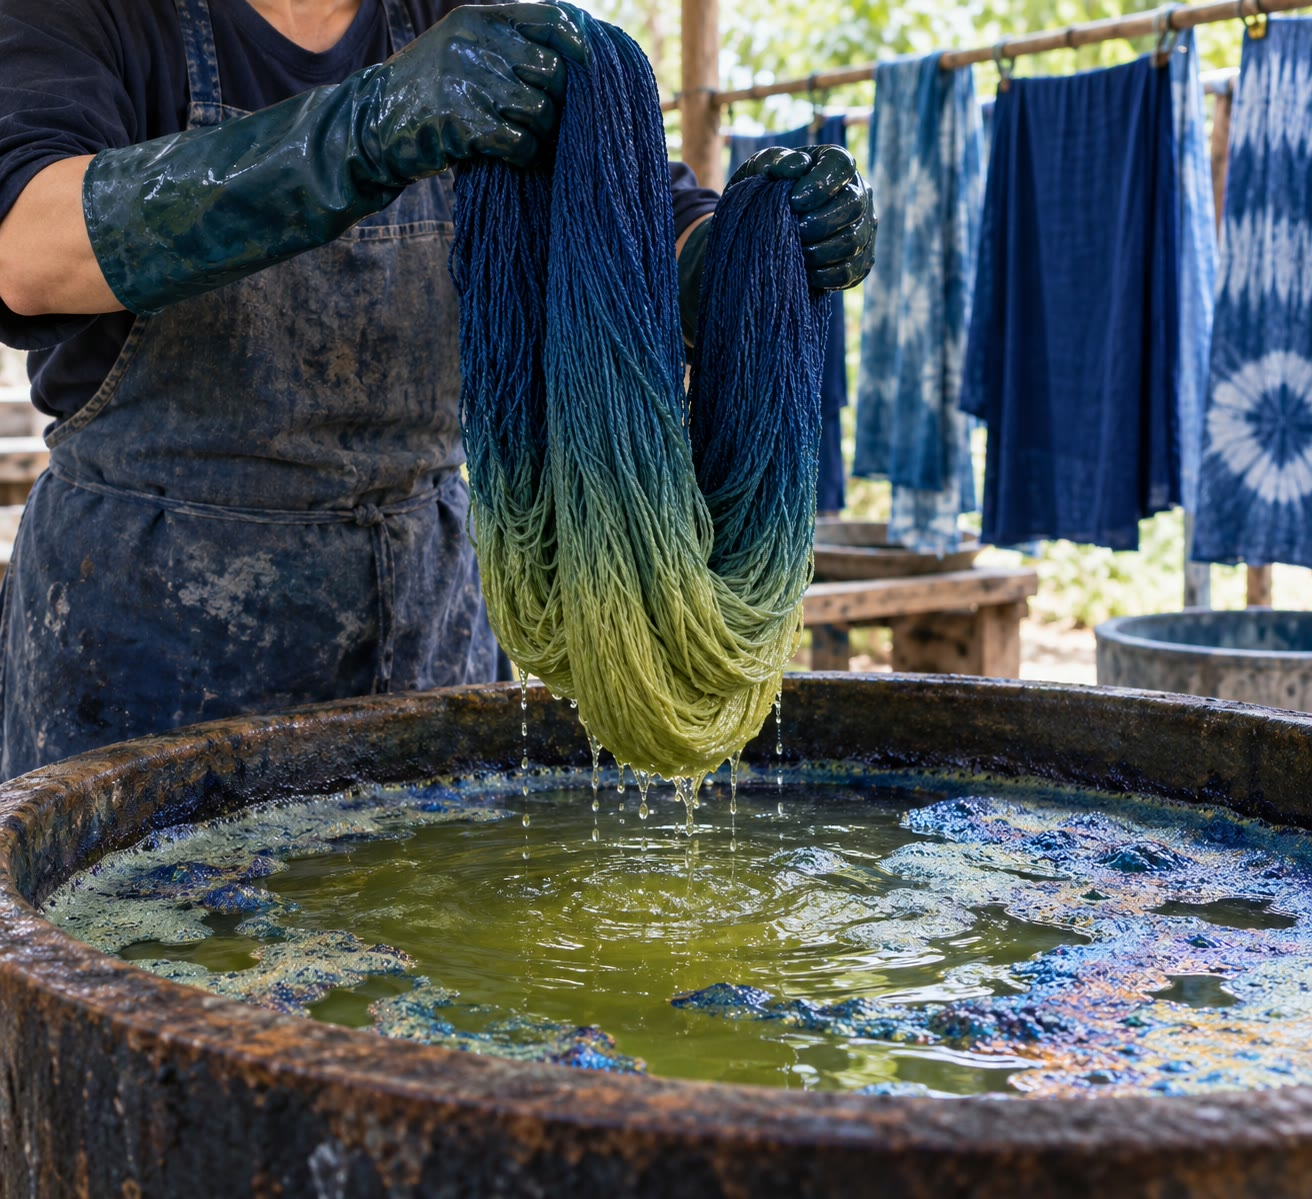
\includegraphics[width=0.55\linewidth]{images/book3/ai/b2-22-indigo-vat-2.jpg}

{\small Dyeing yarn in an indigo vat (illustration). The yarn leaves the vat yellow-green, soaked
in the soluble reduced form of the dye, and turns blue in the air as oxygen turns it back into
insoluble indigo. Indigo, like most dyes, is built on \omterm{def:b2:huckel:aromatic}{aromatic} rings;
the dye industry of the nineteenth century grew from the substitution reactions of this
chapter applied to benzene from coal tar.}
\end{omfigure}

\section{Substitution, not addition}

\begin{definition}[Arene]\label{def:b2:aromatic-substitution:arene}
An \emph{arene}\index{arene} is a hydrocarbon containing at least one \omterm{def:b2:huckel:aromatic}{aromatic} ring, such as
benzene, toluene (methylbenzene) or naphthalene; an aryl group (\ce{Ar}) is an arene less
one hydrogen.
\end{definition}

\begin{proposition}[Why benzene does not add]\label{prop:b2:aromatic-substitution:no-addition}
An addition to benzene would turn the \omterm{def:b2:huckel:aromatic}{aromatic} ring into a \omterm{def:b2:huckel:aromatic}{non-aromatic} cyclohexadiene and
lose most of the \qty{150}{kJ/mol} of \omterm{def:b2:huckel:aromatic}{aromatic} stabilisation; substitution keeps it.
\end{proposition}

\begin{proof}[Argument]
In \cref{ch:b2:huckel}, the hydrogenation of benzene to cyclohexa-1,3-diene was found
\omterm{def:b2:reaction-enthalpy:exothermic}{endothermic} (\qty{+22}{kJ/mol}, from \qty{-206.0}{} and \qty{-227.7}{kJ/mol}), while that of an
ordinary double bond releases \qty{119}{kJ/mol}: the first addition is the costly step.
After the first electrophilic step, the cation formed can either add a nucleophile, which
leaves a \omterm{def:b2:huckel:aromatic}{non-aromatic} \omterm{def:b2:frontier-orbitals:diels-alder}{diene}, or lose a proton, which restores the \omterm{def:b2:huckel:aromatic}{aromatic} ring. The second
path is far more favourable.
% ledger: dfh:C6H6_g, dfh:C6H8_g, dfh:C6H10_g, dfh:C6H12_g
\end{proof}

\section{The mechanism}

\begin{definition}[Electrophilic aromatic substitution]\label{def:b2:aromatic-substitution:seAr}
An \emph{electrophilic aromatic substitution}\index{electrophilic aromatic substitution}
replaces a hydrogen of an \omterm{def:b2:huckel:aromatic}{aromatic} ring by an electrophile \ce{E+}. The electrophile first
bonds to one ring carbon, giving a cation in which that carbon is tetrahedral and the
positive charge is spread over the other five: the \emph{Wheland intermediate}\index{Wheland
intermediate} (an arenium ion). A base then removes the proton from the tetrahedral carbon.
\end{definition}

\begin{proposition}[Two steps]\label{prop:b2:aromatic-substitution:mechanism}
The first step, which destroys the aromaticity, is the slow one; the loss of the proton,
which restores it, is fast.
\end{proposition}

\begin{proof}[Argument]
The \omterm{def:b2:aromatic-substitution:seAr}{Wheland intermediate} is a carbocation stabilised by delocalisation over three carbons
but not \omterm{def:b2:huckel:aromatic}{aromatic}: it lies high above the reactants, and by the Hammond postulate the
transition state leading to it is close to it in structure and energy. The second step
leads down to an \omterm{def:b2:huckel:aromatic}{aromatic} product: its barrier is low.
\end{proof}

\begin{omfigure}
\begin{tikzpicture}
\begin{axis}[width=0.55\linewidth, height=5.4cm, xmin=-0.2, xmax=4.2, ymin=-5.5, ymax=11.5,
  axis x line=bottom, axis y line=left, xtick=\empty, ytick=\empty,
  xlabel={reaction coordinate}, ylabel={energy}, label style={font=\small}, clip=false]
\addplot[omDef, thick] table[x=x, y=sub] {figdata/out/bachelor-2-aromatic-profile.dat};
\addplot[omThm, thick, dashed, restrict x to domain=2:4] table[x=x, y=add] {figdata/out/bachelor-2-aromatic-profile.dat};
\node[font=\scriptsize, anchor=north west] at (axis cs:0.0,-0.6) {\ce{ArH + E+}};
\node[font=\scriptsize, anchor=north] at (axis cs:2,5.7) {Wheland};
\node[font=\scriptsize, anchor=west, omDef] at (axis cs:4.05,-4.0) {\ce{ArE + H+}};
\node[font=\scriptsize, anchor=west, omThm] at (axis cs:4.05,2.0) {addition product};
\node[font=\scriptsize, anchor=south] at (axis cs:1,10.1) {slow};
\end{axis}
\end{tikzpicture}

{\small Energy profile of an \omterm{def:b2:aromatic-substitution:seAr}{electrophilic aromatic substitution}, schematic (a model).
The first step, which forms the \omterm{def:b2:aromatic-substitution:seAr}{Wheland intermediate}, has the highest barrier. Loss of a
proton (solid) restores the \omterm{def:b2:huckel:aromatic}{aromatic} ring; addition of a nucleophile (dashed) would leave a
product above the reactants.}
\end{omfigure}

\begin{omfigure}
\setchemfig{atom sep=2em}
\schemestart
\chemfig{HO-\chemabove{N}{\scriptstyle +}(=[1]O)-[7]\chemabove{O}{\scriptstyle -}} \+ \chemfig{H_2SO_4}
\arrow{<=>}
\chemfig{O=N^{+}=O} \+ \chemfig{HSO_4^{-}} \+ \chemfig{H_2O}
\schemestop

\medskip
\begin{tikzpicture}[font=\small, >={Stealth}]
\tikzset{pics/whel/.style n args={4}{code={
    \foreach \k in {0,...,5} \draw[thick] ({90+60*\k}:0.7) -- ({150+60*\k}:0.7);
    \foreach \k in {#1} \draw[thick] ($({90+60*\k}:0.56)!0.18!({150+60*\k}:0.56)$) -- ($({90+60*\k}:0.56)!0.82!({150+60*\k}:0.56)$);
    \ifnum#2>-1 \node[font=\scriptsize] at ({90+60*#2}:0.36) {$+$};\fi
    \draw[thick] (270:0.7) -- ++(-125:0.42) node[anchor=north east, inner sep=1pt, font=\scriptsize] {H};
    \draw[thick] (270:0.7) -- ++(-55:0.42) node[anchor=north west, inner sep=1pt, font=\scriptsize] {#4};
    \if\relax\detokenize{#3}\relax\else
      \draw[thick] (90:0.7) -- (90:1.1) node[anchor=south, inner sep=1pt, font=\scriptsize] {#3};\fi
  }}}
  \foreach \k in {0,...,5} \draw[thick] ({90+60*\k}:0.7) -- ({150+60*\k}:0.7);
  \foreach \k in {0,2,4} \draw[thick] ($({90+60*\k}:0.56)!0.18!({150+60*\k}:0.56)$) -- ($({90+60*\k}:0.56)!0.82!({150+60*\k}:0.56)$);
  \node at (1.3,0) {$+$};
  \node at (2.0,0) {\ce{NO2+}};
  \draw[->, thick] (2.6,0) -- (3.8,0) node[midway, above, font=\scriptsize] {slow};
  \pic at (4.7,0.1) {whel={1,4}{0}{}{\ce{NO2}}};
  \draw[->, thick] (5.6,0) -- (6.8,0) node[midway, above, font=\scriptsize] {fast} node[midway, below, font=\scriptsize] {$-$\ce{H+}};
  \begin{scope}[xshift=7.7cm]
    \foreach \k in {0,...,5} \draw[thick] ({90+60*\k}:0.7) -- ({150+60*\k}:0.7);
    \foreach \k in {0,2,4} \draw[thick] ($({90+60*\k}:0.56)!0.18!({150+60*\k}:0.56)$) -- ($({90+60*\k}:0.56)!0.82!({150+60*\k}:0.56)$);
    \draw[thick] (270:0.7) -- (270:1.1) node[anchor=north, font=\scriptsize] {\ce{NO2}};
  \end{scope}
\end{tikzpicture}
\par\vspace{6pt}

{\small Nitration of benzene. Sulfuric acid protonates nitric acid, which loses water: the
nitronium ion \ce{NO2+} is the electrophile. It bonds to one carbon (slow), giving the
\omterm{def:b2:aromatic-substitution:seAr}{Wheland intermediate}, whose positive charge is spread over the ring; loss of a proton
(fast) gives nitrobenzene.}
\end{omfigure}

\section{The reactions}

\paragraph{Halogenation.} Bromine or chlorine alone is too weak an electrophile; a Lewis acid
(\ce{FeBr3}, \ce{AlCl3}) polarises the halogen by binding one of its atoms, and the outer
bromine attacks the ring.

\paragraph{Nitration.} A mixture of concentrated nitric and sulfuric acids (above) gives the
nitronium ion.

\paragraph{Sulfonation.} Fuming sulfuric acid (\ce{SO3} in \ce{H2SO4}) gives benzenesulfonic acid.
The reaction is reversible: heating the sulfonic acid in dilute aqueous acid removes the
\ce{SO3H} group again, which makes it a useful temporary blocking group.

\begin{definition}[Friedel--Crafts reactions]\label{def:b2:aromatic-substitution:friedel-crafts}
A \emph{Friedel--Crafts alkylation}\index{Friedel--Crafts alkylation} attaches an alkyl
group to an \omterm{def:b2:huckel:aromatic}{aromatic} ring from a halogenoalkane and a Lewis acid (\ce{AlCl3}). A
\emph{Friedel--Crafts acylation}\index{Friedel--Crafts acylation} attaches an acyl group
\ce{RCO} from an acyl chloride and \ce{AlCl3}, through the \emph{acylium ion}\index{acylium
ion} \ce{R-C#O+}, giving an aryl ketone.
\end{definition}

\begin{proposition}[Limits of the Friedel--Crafts reactions]\label{prop:b2:aromatic-substitution:friedel-crafts-limits}
\omterm{def:b2:aromatic-substitution:friedel-crafts}{Friedel--Crafts alkylation} suffers from rearrangements of the carbocation and from
polyalkylation; acylation stops after one substitution, gives no rearrangement, and needs at
least one equivalent of \ce{AlCl3}. Neither works on a ring bearing a strongly \omterm{def:b2:aromatic-substitution:directing}{deactivating
group}.
\end{proposition}

\begin{proof}[Argument]
The alkylating electrophile is a carbocation (or a polarised complex that behaves like one),
which rearranges to a more stable one by hydride or alkyl shifts: 1-chloropropane gives
mostly isopropylbenzene. An alkyl group activates the ring (next section), so the product
reacts faster than benzene and is alkylated again. The \omterm{def:b2:aromatic-substitution:friedel-crafts}{acylium ion} is stabilised by
resonance (\ce{R-C+=O} $\leftrightarrow$ \ce{R-C#O+}) and does not rearrange; the acyl group
deactivates the ring, so the product does not react further; and the ketone formed binds
\ce{AlCl3} through its oxygen, removing the catalyst from the reaction: one equivalent is
consumed. A strongly deactivated ring is too poor a nucleophile for these weak electrophiles.
\end{proof}

\section{Substituent effects}

\begin{definition}[Directing groups]\label{def:b2:aromatic-substitution:directing}
A substituent on a benzene ring is an \emph{activating group}\index{activating group} if the
ring reacts faster than benzene, a \emph{deactivating group}\index{deactivating group} if it
reacts more slowly. It is an \emph{ortho/para director}\index{ortho/para director} if the new
group enters mainly at the positions next to it and opposite to it, a \emph{meta
director}\index{meta director} if it enters mainly at the positions once removed.
\end{definition}

\begin{proposition}[Donors and acceptors]\label{prop:b2:aromatic-substitution:directing}
Groups donating electrons to the ring by mesomeric effect (\ce{-OH}, \ce{-OCH3}, \ce{-NH2},
\ce{-NHCOCH3}) or by inductive effect and \omterm{def:b2:fragment-orbitals:hyperconjugation}{hyperconjugation} (alkyls) activate the ring and direct
ortho/para. Groups withdrawing electrons by mesomeric effect (\ce{-NO2}, \ce{-CN}, \ce{-COR},
\ce{-COOH}, \ce{-SO3H}) deactivate it and direct meta.
\end{proposition}

\begin{proof}
Compare the \omterm{def:b2:aromatic-substitution:seAr}{Wheland intermediates}. For attack ortho or para to a substituent G, one of the
three resonance structures puts the positive charge on the carbon bearing G; for attack meta,
none does. A donor G (a lone pair on O or N) stabilises a positive charge on the carbon it is
attached to, adding a fourth resonance structure in which every atom has an octet: the ortho
and para intermediates are lowered, and by the Hammond postulate so are the transition states
leading to them. An acceptor G destabilises a positive charge on its carbon: the ortho and para
intermediates are raised, and attack meta, which avoids that structure, is the least
disfavoured, though slower than on benzene.
\end{proof}

\begin{omfigure}
\begin{tikzpicture}[font=\small]
\tikzset{pics/whel/.style n args={4}{code={
    \foreach \k in {0,...,5} \draw[thick] ({90+60*\k}:0.7) -- ({150+60*\k}:0.7);
    \foreach \k in {#1} \draw[thick] ($({90+60*\k}:0.56)!0.18!({150+60*\k}:0.56)$) -- ($({90+60*\k}:0.56)!0.82!({150+60*\k}:0.56)$);
    \ifnum#2>-1 \node[font=\scriptsize] at ({90+60*#2}:0.36) {$+$};\fi
    \draw[thick] (270:0.7) -- ++(-125:0.42) node[anchor=north east, inner sep=1pt, font=\scriptsize] {H};
    \draw[thick] (270:0.7) -- ++(-55:0.42) node[anchor=north west, inner sep=1pt, font=\scriptsize] {#4};
    \if\relax\detokenize{#3}\relax\else
      \draw[thick] (90:0.7) -- (90:1.1) node[anchor=south, inner sep=1pt, font=\scriptsize] {#3};\fi
  }}}
  \node[anchor=east] at (-1.0,0) {methoxy, para attack:};
  \pic at (0,0) {whel={1,4}{0}{\ce{OCH3}}{E}};
  \node at (1.25,0.1) {$\leftrightarrow$};
  \begin{scope}[xshift=2.5cm]
    \foreach \k in {0,...,5} \draw[thick] ({90+60*\k}:0.7) -- ({150+60*\k}:0.7);
    \foreach \k in {1,4} \draw[thick] ($({90+60*\k}:0.56)!0.18!({150+60*\k}:0.56)$) -- ($({90+60*\k}:0.56)!0.82!({150+60*\k}:0.56)$);
    \draw[thick] (-0.06,0.7) -- (-0.06,1.1); \draw[thick] (0.06,0.7) -- (0.06,1.1);
    \node[anchor=south, inner sep=1pt, font=\scriptsize] at (0,1.1) {$\overset{+}{\mathrm O}\mathrm{CH_3}$};
    \draw[thick] (270:0.7) -- ++(-125:0.42) node[anchor=north east, inner sep=1pt, font=\scriptsize] {H};
    \draw[thick] (270:0.7) -- ++(-55:0.42) node[anchor=north west, inner sep=1pt, font=\scriptsize] {E};
  \end{scope}
  \node[anchor=west, font=\scriptsize] at (3.4,0) {extra structure, every atom with an octet};
  \begin{scope}[yshift=-3.5cm]
    \node[anchor=east] at (-1.0,0) {nitro, para attack:};
    \pic at (0,0) {whel={1,4}{0}{\ce{NO2}}{E}};
    \node[anchor=west, font=\scriptsize] at (1.0,0) {positive charge on the carbon bearing the acceptor};
  \end{scope}
\end{tikzpicture}

{\small \omterm{def:b2:aromatic-substitution:seAr}{Wheland intermediates} for attack para to a substituent. With methoxy, a lone pair of
oxygen shares the positive charge (an extra resonance structure, all atoms with an octet):
the intermediate is stabilised, the substituent is activating and ortho/para directing. With
nitro, one structure places the positive charge on the carbon bearing the electron-withdrawing
group: the intermediate is destabilised, and attack goes meta.}
\end{omfigure}

\begin{proposition}[Halogens]\label{prop:b2:aromatic-substitution:halogens}
Halogen substituents deactivate the ring but direct ortho/para.
\end{proposition}

\begin{proof}[Argument]
Their inductive withdrawal (electronegativity) lowers the electron density of the whole ring
and slows every attack: deactivating. But a lone pair of the halogen can still share the
positive charge of the ortho and para \omterm{def:b2:aromatic-substitution:seAr}{Wheland intermediates}, which the meta intermediate cannot
use: among the slower attacks, ortho and para remain the least slow.
\end{proof}

\section{Polysubstituted benzenes}

\begin{method}[Predicting the position of substitution]\label{met:b2:aromatic-substitution:predict-position}
\begin{enumerate}
  \item For each substituent, mark the positions it favours (ortho/para or meta).
  \item If they agree, that position wins. If they disagree, the stronger activator decides
        (\ce{-NH2}, \ce{-OH} $>$ \ce{-OCH3} $>$ \ce{-NHCOCH3} $>$ alkyl $>$ halogen).
  \item Avoid the position between two substituents in a 1,3-relationship (hindered), and
        expect para over ortho when the groups are bulky.
\end{enumerate}
\end{method}

\begin{method}[Planning an aromatic synthesis]\label{met:b2:aromatic-substitution:plan-aromatic}
\begin{enumerate}
  \item Choose the order of the steps so that each group already present directs the next one
        where it is wanted: to make 3-bromonitrobenzene, nitrate first (\omterm{def:b2:aromatic-substitution:directing}{meta director}), then
        brominate; to make 4-bromonitrobenzene, brominate first.
  \item Use convertible groups: an acyl group (meta) can be reduced to an alkyl (ortho/para);
        a nitro group (meta) reduced to an amine (ortho/para); an alkyl oxidised to
        \ce{-COOH} (meta).
  \item Block a position with \ce{-SO3H} and remove it at the end.
  \item Tame a strong activator: an amine is acylated (\ce{-NHCOCH3}) before nitration or
        halogenation, then freed again.
\end{enumerate}
\end{method}

\begin{history}[Friedel and Crafts]
\begin{minipage}[t]{0.18\linewidth}
\vspace{0pt}
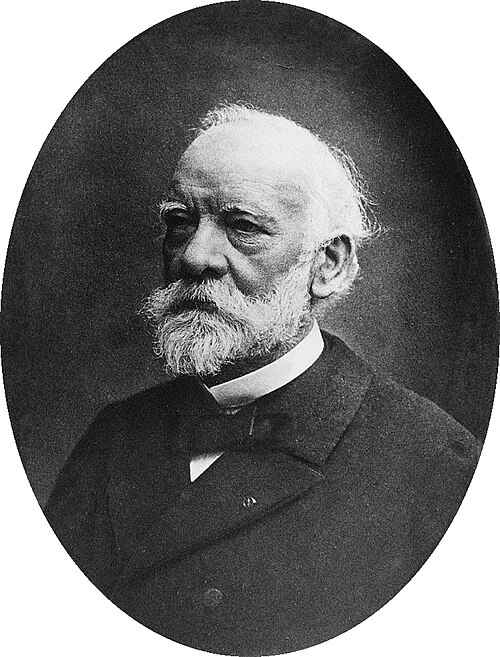
\includegraphics[width=\linewidth]{images/book3/friedel.jpg}
\end{minipage}\hspace{0.02\linewidth}%
\begin{minipage}[t]{0.18\linewidth}
\vspace{0pt}
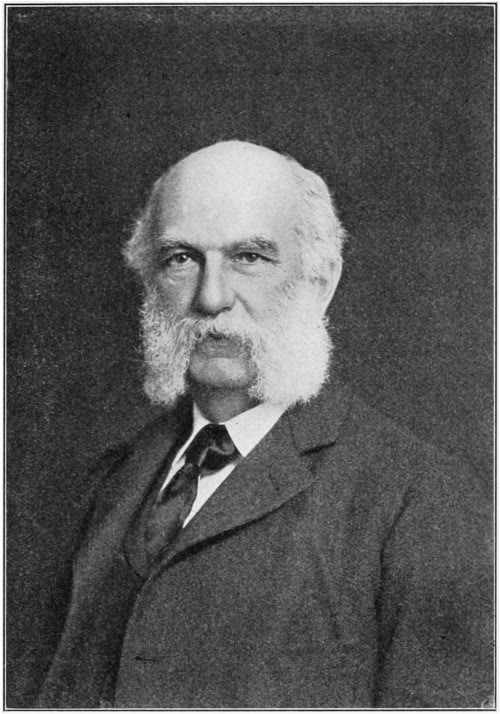
\includegraphics[width=\linewidth]{images/book3/crafts.jpg}
\end{minipage}\hfill
\begin{minipage}[t]{0.58\linewidth}
\vspace{0pt}
In 1877 Charles Friedel and James Mason Crafts, working together in Paris, found that
aluminium chloride makes halogenoalkanes and acyl chlorides react with benzene. Their
reactions became the standard way to attach carbon groups to \omterm{def:b2:huckel:aromatic}{aromatic} rings, and the Lewis
acid catalysis they discovered reached far beyond it. (Portraits: Friedel, 1890s; Crafts, from
\textit{Popular Science Monthly}, 1900; public domain, Wikimedia Commons.)
\end{minipage}
\end{history}

\begin{safety}{\ghs[5mm]{GHS02}\,\ghs[5mm]{GHS05}\,\ghs[5mm]{GHS06}\,\ghs[5mm]{GHS08}}
Benzene is a carcinogen and is replaced by toluene or other \omterm{def:b2:aromatic-substitution:arene}{arenes} wherever possible.
Concentrated nitric and sulfuric acids are corrosive and the nitrating mixture is strongly
oxidising; it is cooled and the \omterm{def:b2:aromatic-substitution:arene}{arene} added slowly, since nitrations are \omterm{def:b2:reaction-enthalpy:exothermic}{exothermic}.
Bromine is very toxic and corrosive; aluminium chloride reacts violently with water. Nitroarenes
are toxic.
% ledger: ghs:benzene, ghs:toluene, ghs:HNO3, ghs:H2SO4, ghs:Br2, ghs:AlCl3, ghs:nitrotoluene-4
\end{safety}

\section{Exercises}

\begin{exercise}[$\star$]\label{exo:b2:aromatic-substitution:1}
Write the formation of the nitronium ion from nitric acid and sulfuric acid.
\end{exercise}

\begin{exercise}[$\star$]\label{exo:b2:aromatic-substitution:2}
Give the main products of the bromination (\ce{Br2}, \ce{FeBr3}) of toluene and of
nitrobenzene.
\end{exercise}

\begin{exercise}[$\star$]\label{exo:b2:aromatic-substitution:3}
Classify as activating or deactivating, ortho/para or meta: \ce{-CH3}, \ce{-OH}, \ce{-Cl},
\ce{-NO2}, \ce{-COCH3}, \ce{-NHCOCH3}.
\end{exercise}

\begin{exercise}[$\star$]\label{exo:b2:aromatic-substitution:4}
Give the product of benzene with ethanoyl chloride and aluminium chloride.
\end{exercise}

\begin{exercise}[$\star\star$]\label{exo:b2:aromatic-substitution:5}
Benzene and 1-chloropropane with \ce{AlCl3} give mainly isopropylbenzene. Explain, and give a
two-step route to propylbenzene.
\end{exercise}

\begin{exercise}[$\star\star$]\label{exo:b2:aromatic-substitution:6}
Phenol decolourises bromine water at once, without a catalyst, giving
2,4,6-tribromophenol. Explain.
\end{exercise}

\begin{exercise}[$\star\star$]\label{exo:b2:aromatic-substitution:7}
Give syntheses of 3-bromonitrobenzene and 4-bromonitrobenzene from benzene.
\end{exercise}

\begin{exercise}[$\star\star$]\label{exo:b2:aromatic-substitution:8}
Aniline is nitrated poorly (oxidation, and meta product), but acetanilide gives mainly
4-nitroacetanilide. Explain both facts.
\end{exercise}

\begin{exercise}[$\star\star$]\label{exo:b2:aromatic-substitution:9}
Show how a sulfonic acid group can be used to prepare 2-bromotoluene free of its para isomer.
\end{exercise}

\begin{exercise}[$\star\star\star$]\label{exo:b2:aromatic-substitution:10}
Where does 4-methylanisole (4-methoxytoluene) undergo nitration? Explain with the two
directing groups.
\end{exercise}

\begin{exercise}[$\star\star\star$]\label{exo:b2:aromatic-substitution:11}
2,4,6-Trinitrotoluene is made by three successive nitrations of toluene, each under harsher
conditions. Explain why.
\end{exercise}

\begin{exercise}[$\star\star\star$]\label{exo:b2:aromatic-substitution:12}
Propose a synthesis of 4-nitrobenzoic acid from toluene, and of 3-nitrobenzoic acid.
\end{exercise}

\section{Problem: Nitrating Toluene}

\begin{problem}[{Weekend problem --- the nitronium ion and the mechanism of nitration, the
ortho, meta and para positions of toluene against the statistical ratio, the separation of the
isomers, and a mass balance}]
\label{pb:b2:aromatic-substitution:1}
Data: melting points: 2-nitrotoluene \qty{-10}{\degreeCelsius}, 3-nitrotoluene
\qty{16}{\degreeCelsius}, 4-nitrotoluene \qty{52}{\degreeCelsius}. Exercise data for a run:
\qty{100}{g} of toluene, \omterm{def:b2:continuous-reactors:conversion}{conversion} 90~\%, isomer distribution 58~\% ortho, 4~\% meta,
38~\% para. Molar masses (\unit{g/mol}): C 12.011, H 1.008, N 14.007, O 15.999.
% ledger: mp:2-nitrotoluene, mp:3-nitrotoluene, mp:4-nitrotoluene, aw:C, aw:H, aw:N, aw:O

\medskip
\noindent\textbf{Part I --- The electrophile and the mechanism.}
\begin{enumerate}
  \item Write the formation of the nitronium ion.
  \item Draw its Lewis structure and give its shape.
  \item Write the attack of \ce{NO2+} on toluene para to the methyl.
  \item Draw the three resonance structures of the para \omterm{def:b2:aromatic-substitution:seAr}{Wheland intermediate}.
  \item Which step is rate-determining?
  \item What removes the proton in the second step?
\end{enumerate}

\medskip
\noindent\textbf{Part II --- The three positions.}
\begin{enumerate}[resume]
  \item How many ortho, meta and para positions has toluene?
  \item What ratio would a random attack give?
  \item Draw the meta \omterm{def:b2:aromatic-substitution:seAr}{Wheland intermediate} and explain why it is the least stabilised.
  \item How does the methyl group stabilise the ortho and para intermediates?
  \item Compare the observed ratio with the statistical one: which positions are favoured?
  \item Compare the yield per position at ortho (half of the ortho percentage) and at para.
        Suggest a reason for the difference.
  \item Is toluene nitrated faster or more slowly than benzene?
\end{enumerate}

\medskip
\noindent\textbf{Part III --- Separation.}
\begin{enumerate}[resume]
  \item Which isomer is solid at room temperature?
  \item Suggest how to isolate it from the mixture by cooling.
  \item Why does symmetry favour a high melting point?
  \item How could the ortho and meta isomers be separated afterwards?
  \item Why are these isomers hard to separate by simple distillation?
\end{enumerate}

\medskip
\noindent\textbf{Part IV --- Mass balance.}
\begin{enumerate}[resume]
  \item Compute the molar mass of toluene and of nitrotoluene.
  \item Compute the amount of toluene and of nitrotoluene formed.
  \item Compute the masses of the three isomers.
  \item What further reaction must be avoided by cooling and by not using excess acid?
  \item How would you make 4-nitrobenzoic acid from the para isomer?
  \item State the mass of 4-nitrotoluene obtained from \qty{100}{g} of toluene in this run.
\end{enumerate}
\end{problem}
